\chapter*{Введение}
\addcontentsline{toc}{chapter}{Введение}


В последние годы наблюдается заметный рост количества уязвимостей в программном обеспечении. Так, согласно статистике \cite{CVEstats}, в $2016$ году было обнаружено $6447$ уязвимостей, в $2017$ ~---  $14714$, a в $2018$ ~--- $16555$. Это связано как с объемом и сложностью, разрабатываемого программного обеспечения, так и с развитием техник тестирования безопасности.

\begin{figure}[h]
    \center{
        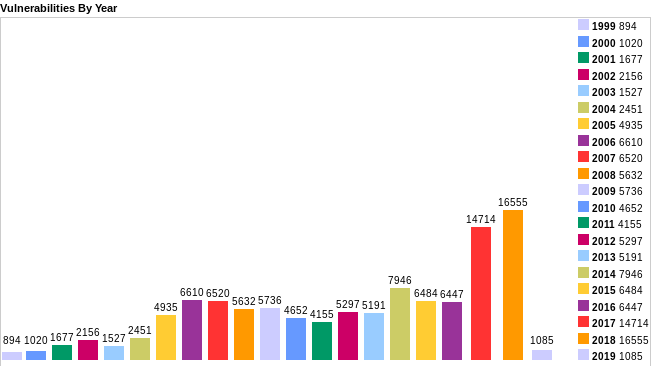
\includegraphics[scale=0.5]{img/cve_stats.png}
    }
    \caption{Статистика опубликованных уязвимостей за последние $20$ лет}
    \label{fig:image}
\end{figure}

Одним из популярных подходов к автоматизации поиска уязвимостей является фаззинг-тестирование. Это
техника тестирования программного обеспечения, заключающая в автоматической генерации входных данных. Целью фаззинга является нахождение таких входных данных, которые вызовут аварийное завершение программы.

Для достижения своей цели фаззеру необходимо генерировать входные данные, позволяющие пройти по разным путям выполнения. Один из популярных подходов, впервые примененный в AFL \cite{AFL} заключается в мутировании изначальных входных данных с целью увеличения покрытия.

Несмотря на высокую эффективность такого подхода он не лишен недостатков. Так например в листинге \ref{lst:example1}
\begin{lstlisting}[environoment=C_LANG, caption=example.c, captionpos=b, label={lst:example1}]
uint32_t buf[10];
read(10, &buf, 40);
buf[0] &= 500;

if (buf[0] == 100) {
    //branch 1
    ...
} else {
    //branch 2
    ...
}
\end{lstlisting}

для того, чтобы найти входные данные для прохождения по ветке $1$ необходимо фактически перебрать $2^{32}$ значений. Для решения подобных проблем в \cite{DRILLER} предлагается подход, основанный на динамическом символьном выполнении. В случае если фаззер не может сгенерировать входные данные для прохождения по некоторой ветке в течение некоторого ограниченного времени, запускается модуль символьного выполнения, который составляет и решает предикат пути. Затем фаззер продолжает свою работу.
Подход из \cite{DRILLER} реализован в инструменте \texttt{DRILLER}, распространяемом под открытой лицензией.

Комбинирование фаззинга и символьного выполнения тоже имеет свои сложности:
\begin{itemize}
    \item Генерация формул для каждой инструкции достаточно времязатратная операция.
    \item Задача поиска решений символьных уравнений является \textbf{NP полной}, не смотря на наличие множества эвристик невозможно гарантировать решение предиката пути за разумное время.
\end{itemize}

В данной работе предлагается иной способ улучшения эффективности открытия фаззером новых путей. В примере из листинга \ref{lst:example1} фаззер не знает от каких входных данных зависит условный переход и может мутировать все байты входного файла для открытия ветки $1$, однако в действительности значение \textbf{buf[0]} определяется только одним байтом, и только его и имеет смысл мутировать.
Так если у фаззера будет возможность для каждого условного перехода узнать от каких входных данных зависит его выполнение, это позволит существенно сократить количество итераций, необходимых для открытия пути.

Предметом работы является исследование и разработка методов, позволяющих предоставить фаззеру искомую информацию.

Целью работы является:
\begin{itemize}
    \item Исследовать методы динамического анализа с целью выявления подходов, применимых к задаче определения входных данных, влияющищих на выполнение условных переходов.
    \item Провести анализ существующих инструментов динамического анализа с точки зрения применимости к решаемой задаче.
    \item Привести программную реализацию исследованных методов, провести её тестирование на наборе \texttt{LAVA} и программах с открытым исходным кодом.
\end{itemize}


В первой главе работы содержится обзор предметной области. Описываются предмет и методы динамического анализа. Дается обзор инструментов динамической бинарной инструментации, технологий динамического символьного выполнения и динамического анализа помеченных данных, а также существующих инструментов, использующих эти технологии.

Во второй главе описываются предлагаемые методы решения поставленной задачи.

В третьей главе проводится сравнение существующих инструментов с целью выбора базы для дальнейшей работы.

В четвертой главе описывается реализация предложенных методов.



\chapter{Обзор}

% \chapter{Методы реализации динамического анализа}

\section{Динамический Анализ}

Динамический анализ - это анализ, происходящий во время выполнение программы. Однако, просто запустить программу может быть недостаточно. Существует несколько способов получения дополнительной информации во время выполнения:

\begin{itemize}
\item {\em Исполнение кода в виртуальном окружении}. При данном подходе программа запускается внутри некоторого программного эмулятора. Например qemu \cite{QEMU}.
%\item $\sigma$ is a {\em symbolic store} that associates program variables with expressions over \mynote{[D] $\alpha_i$ also concrete?} concrete and symbolic values $\alpha_i$.

\item {\em Статическая инструментация}.
Статическая инструментация бывает двух видов.
    \begin{itemize}
        \item \texttt{Статическая инструментация исходного кода}. В случае, если имеется доступ к исходному коду, можно просто внести изменения в текстовые файлы с кодом. Добавление отладочной печати может быть примером статической инструментации исходного кода. Подобный вид инструментации также поддерживается непосредственно компилятором. Так GCC имеет опцию  \texttt{-finstrument-functions}
        \item \texttt{Статическая инструментация бинарного кода (SBI)}. В случае отсутствия исходного кода, изменениям может быть подвержен сам исполняемый файл на диске. Тривиальным примером такой инструментации может быть например замена условных переходов на \texttt{nop} инструкции. 
    \end{itemize}

\item {\em Динамическая бинарная инструментация}. Данный вид инструментации позволяет вносить изменения в программу непосредственно в процессе её выполнения. Подробное описание возможных подходов к реализации динамической инструментации можно найти в \cite{PBA}.
\end{itemize}

В данной работе проводилось исследование инструментов, основанных на использовании эмуляторов и динамической бинарной инструментации.


\section{Динамическая бинарная инструментация}

Основная идея динамической бинарной инструментации (DBI) заключается в том, что инструментирующая программа контролирует все выполняемые инструкции. Классическая реализация работает следующим образом. Перед непосредственным запуском программы происходит настройка модуля динамической инструментации и устанавливаются функции обратного вызова для различных видов событий, затем код инструментируемой программой считывается по базовым блокам и выполняется.

Рассмотрим несколько популярных DBI инструментов.

\subsection{QDBI}

В \cite{QDBI} \texttt{QDBI} - расшифровывается как \texttt{QuarkslaB Dynamic binary Instrumentation}, авторы позиционируют его как кросплатформенный и кросс-архитектурный фреймворк динамической бинарной инструментации. В планах разработчиков поддержка операционных систем Linux, macOS, Android, iOS и Windows, а также архитектур  x86, x86-64, ARM и AArch64.

Однако, в настоящий момент полноценно поддерживаются только Linux, macOS, Windows на x86-64 архитектуре, при этом поддержки SIMD инструкций нет.

Согласно \cite{QDBI} архитектура \texttt{QDBI} описывается следующей схемой.
\begin{figure}[H]
    \center{
        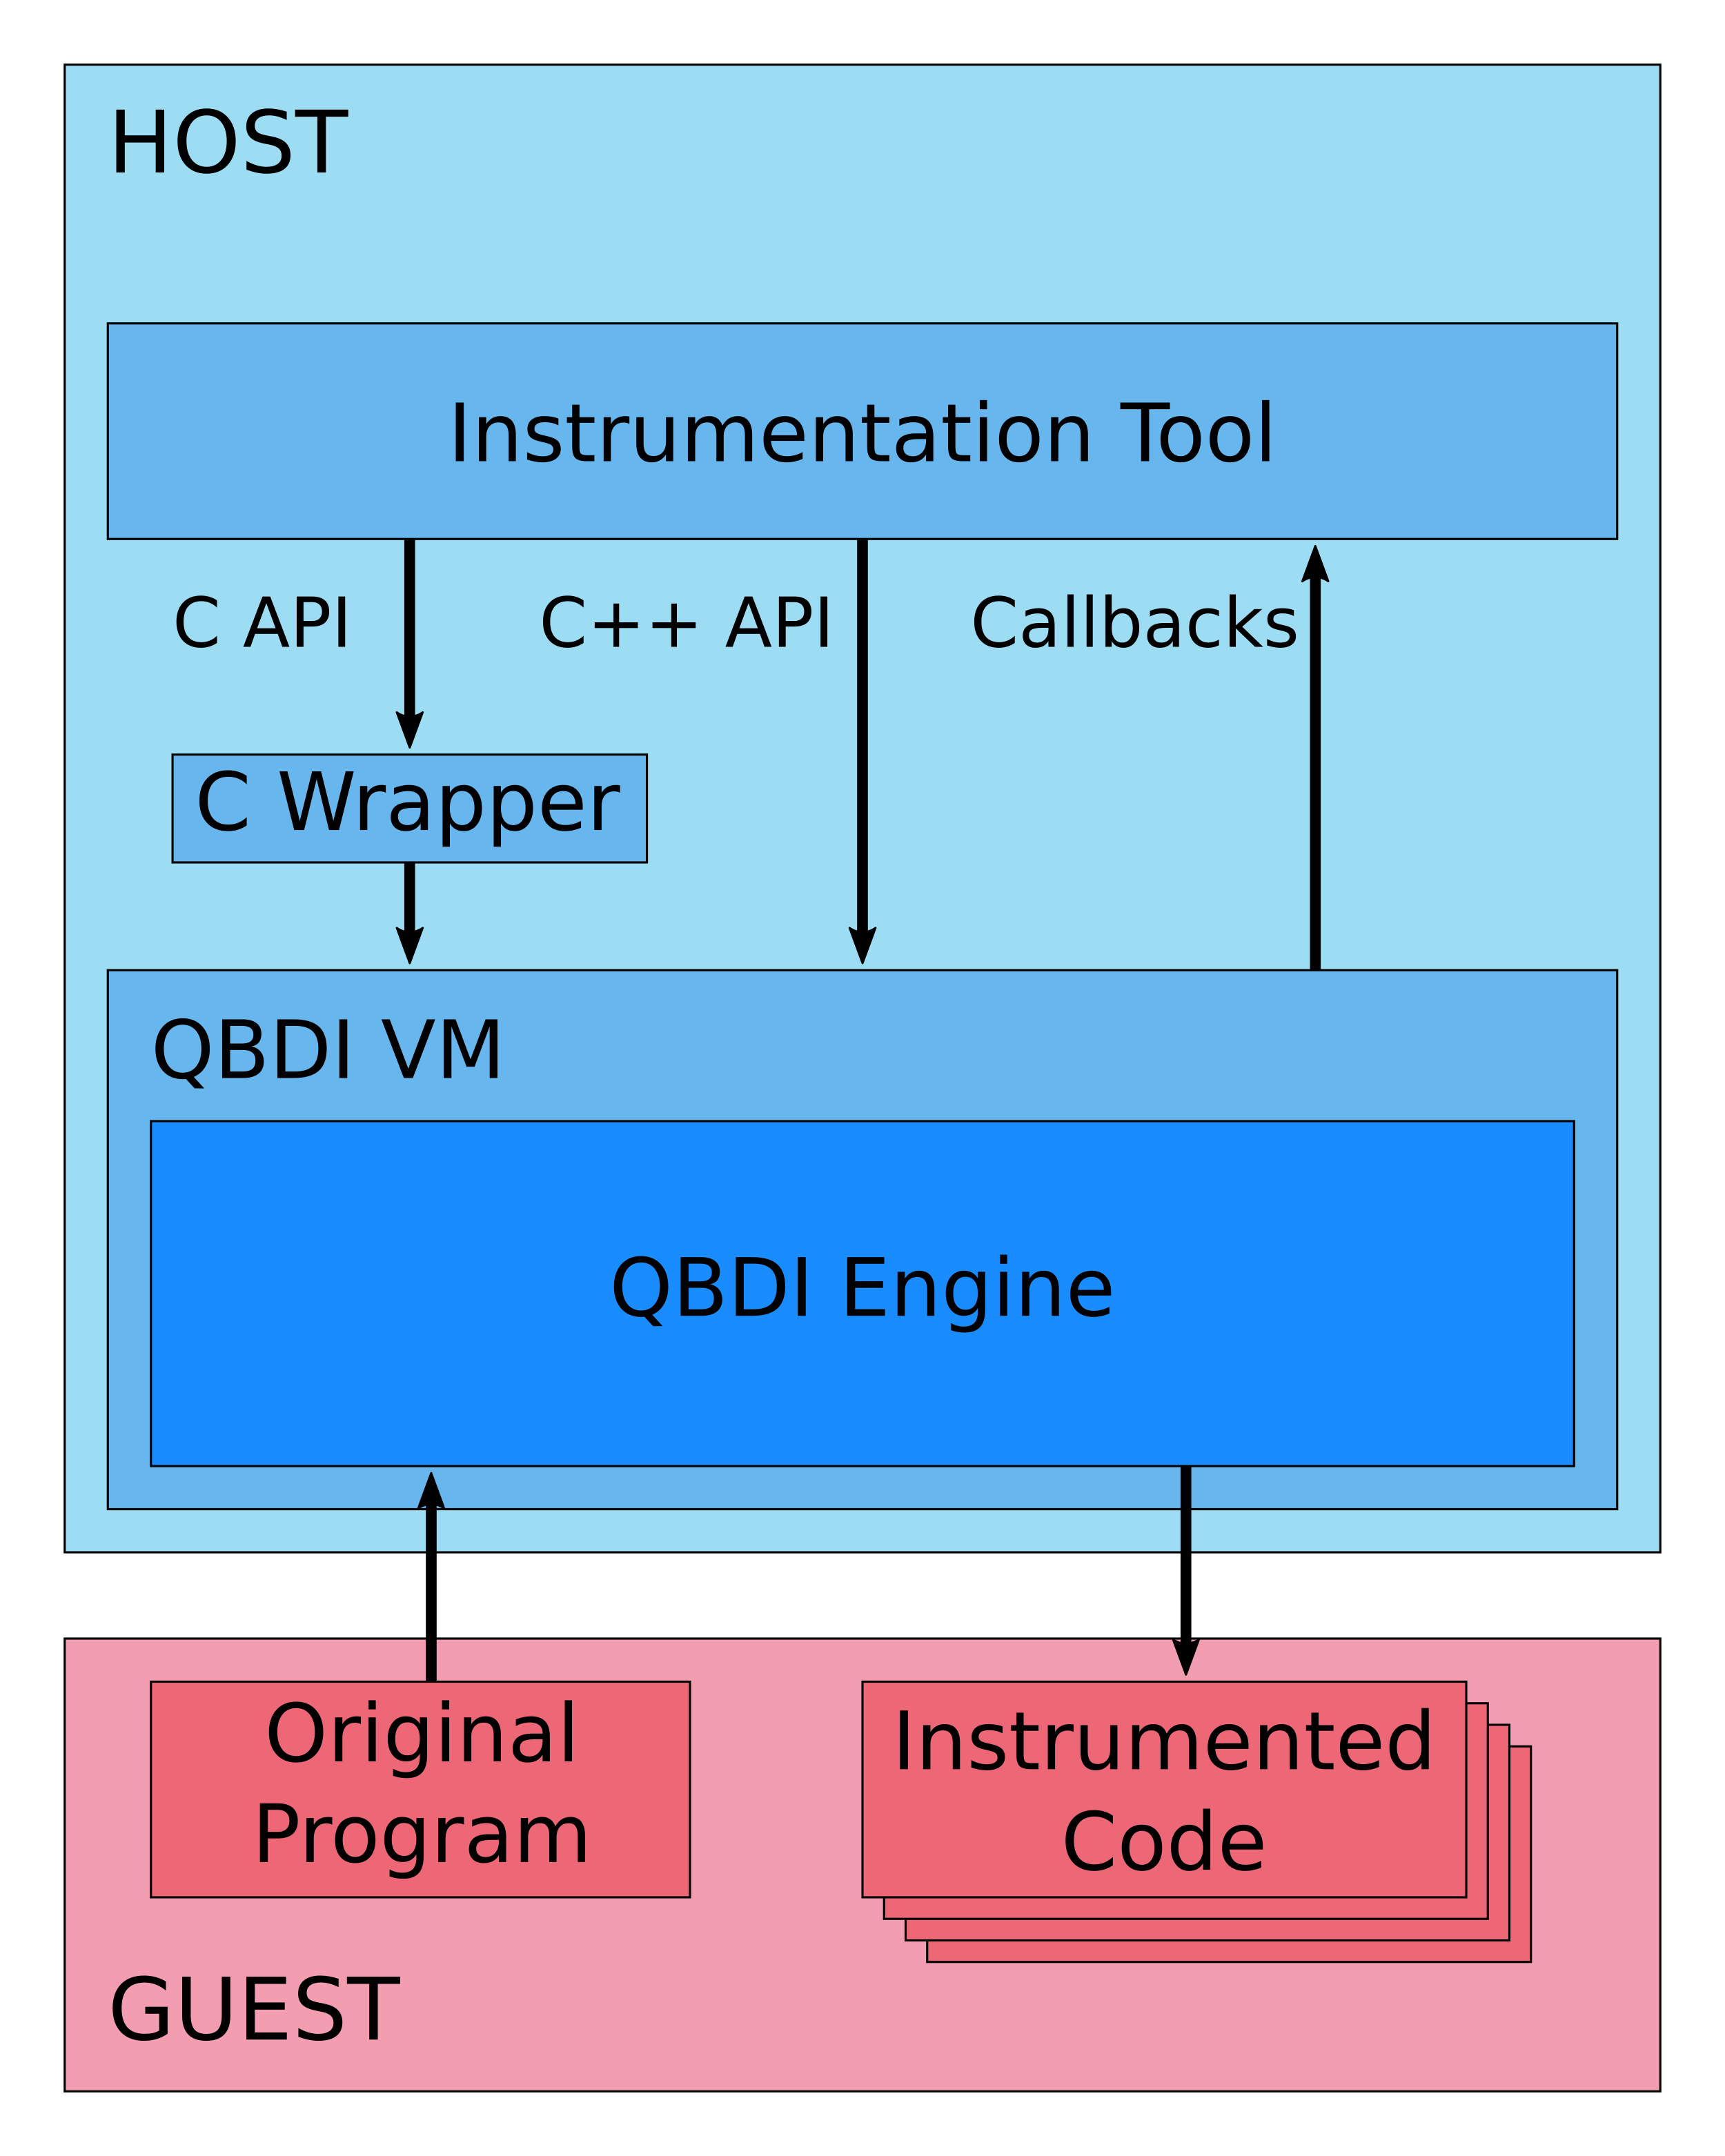
\includegraphics[scale=0.5]{img/qdbi_architecture.png}
    }
    \caption{Архитектура QDBI}
    \label{fig:qdbi}
\end{figure}

В качества хоста выступает пользовательская программа инструментации, написанная с использованием QDBI API, которое позволяет установить функции обратного вызова для различных событий.

\texttt{QDBI} представляет из себя модуль, управляющий выполнением оригинальной программы. Он считывает в цикле код следующего базового блока, а затем при помощи JIT генерирует его пропатченную версию вместе с кодом инструментации. Все это происходит в одном адресном пространстве, что ограничивает возможности QDBI. В частности он не позволяет инструментировать код загрузчика.

QDBI может использоваться двумя принципиально различными способами. В первом случае предполагается наличие исходного кода. В таком случае есть возможность проводить анализ не только программы целиком, но и отдельных функций, предварительно сформировав окружение. При этом фактически производится статическая инструментация исходного кода вручную.

Другой вариант работы более универсален. Инструментирующая программа пишется как отдельной приложение, а фактическая инструментация происходит посредством добавления \texttt{QDBI} библиотеки в texttt{LD\_PRELOAD}.

Поскольку \texttt{QDBI} является достаточно молодым фреймворком, в настоящий момент известных инструментов, написанных на его основе не существует.


\subsection{Valgrind}

\texttt{Valgrind} это достаточно известный фреймворк динамической бинарной инструментации, обычно используется разработчиками для поиска утечек памяти. Был разработан Николасом Нетеркотом в рамках его работы над PHD диссертацией. Хорошее описание фреймворка его особенностей и устройства можно найти в \cite{VALGRIND}.


\texttt{Valgrind} делится на ядро и модули, где собственно ядро предоставляет возможности для бинарной инструментации, а модули представляют собой конкретные инструменты с некоторым функционалом, работающие с API ядра. Одним из наиболее популярных модулей является \texttt{memcheck} - инструмент для поиска утечек памяти.

Ядро \texttt{Valgrind} считывает инструкции инструментируемого приложения и транслирует их в промежуточный язык (IL), \texttt{VEX}. Трансляция производится по базовым блокам, для оттранслированного базового блока вызывается функция инструментации, являющаяся частью запущенного модуля, затем ядром производится JIT компиляция и выполнение полученного кода.

\texttt{Valgrind} поддерживает следующие платформы.

\begin{itemize}

    \item x86/Linux: Отсутствует поддержка SSE4, AVX, AVX2 инструкций.
    \item AMD64/Linux: Поддерживаются все инструкции, включая AVX2.
    \item PPC32/Linux, PPC64/Linux, PPC64LE/Linux
    \item S390X/Linux: Поддерживается
    \item ARM/Linux: Поддерживается начиная с ARMv7.
    \item ARM64/Linux: Поддерживается начиная с ARMv8.
    \item MIPS32/Linux, MIPS64/Linux
    \item X86/Solaris, AMD64/Solaris, X86/illumos, AMD64/illumos: Поддержка начиная с Solaris 11.
    \item X86/Darwin (10.10, 10.11), AMD64/Darwin (10.10, 10.11)
    \item ARM/Android, ARM64/Android, MIPS32/Android, X86/Android:
\end{itemize}

\emph{x86/FreeBSD}, \emph{x86/NetBSD} и \emph{sparc64/Linux} поддерживаются сторонними разработчиками.

Как и \emph{QDBI}, \emph{Valgrind} работает в одном адресном пространстве с инструментируемым приложением. Кроме того, поскольку загрузка осуществляется самим \emph{Valgrind} модули должны быть собраны без использования динамических библиотек.

\subsection{Pin}

\texttt{Pin} ~--- это свободно распространяемый фреймворк для динамической бинарной инструментации с закрытым исходным кодом, подробно прочитать о его устройстве можно в \cite{PIN} или \cite{PBA}.

Pin поддерживает x86 и amd64 архитектуры и работает на операционных системах Linux, Windows и macOS. Pin принимает на вход исполняемый файл и последовательно считывает из него инструкции, затем при необходимости инструментирует их, компилирует при помощи JIT компилятора и выполняет.

Инструменты написанные на основе Pin называются pintools. Pin предоставляет API основанный на функциях обратного вызова. При этом концептуально инструментация в pin состоит из двух частей

\begin{itemize}
    \item Принятие решения какой код куда следует вставить. (\emph{Инструментирующий код})
    \item Пользовательский код, вставляемый в точках, определенных в прошлом пункте (\emph{Анализирующий код})
\end{itemize}

Соответственно к инструментирующему коду относится код, отвечающий за установку функций обратного вызова при наступлении некоторых событий, а к анализирующему коду относятся непосредственно функции обратного вызова.

Выгодно отличает Pin от рассмотренных ранее инструментов бинарной инструментации достаточно богатое API, предоставляющее большее количество событий, на которые можно установить свои обработчики. В частности, вместе с Pin поставляется дизассемблер \emph{Xed}, благодаря которому есть возможность программно извлекать информацию о семантике инструкций.

Pin поддерживает разные уровни гранулярности для инструментации, так можно поставить свой обработчик на всю трассу выполнения, на базовый блок, или на конкретную инструкцию. При этом следует учитывать, что базовый блок с точки зрения Pin может не быть таким на самом деле, поскольку нет возможности определить существуют ли переходы в середину предполагаемого базового блока.

Pin позволяет также инструментировать процесс загрузки кода, вызывая обработчики на загрузку динамических библиотек.

Графическое представление архитектуры Pin можно найти в \cite{PIN}.
\begin{figure}[H]
    \center{
        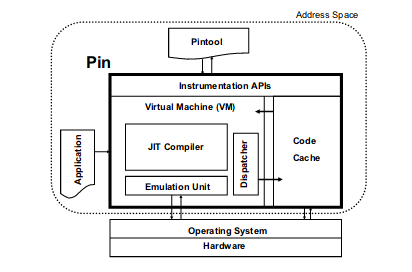
\includegraphics[scale=1]{img/pin_architecture.png}
    }
    \caption{Архитектура Pin}
    \label{fig:pin}
\end{figure}
% Не смотря на возраст статьи иллюстрация \ref{fig:pin} остается актуальной.


Следует отметить, что в настоящий момент актуальны две версии Pin, старая 2015 года выпуска $2.14$ и новая $3.7$. При этом для версии Pin $2.14$ не гарантируется корректная работа на версиях ядра Linux 4 и старше, с другой стороны новые версии Pin используют \texttt{Pin Crt} (Pin C Runtime) вместо системных библиотек, что накладывает определенные ограничения на pintools:

\begin{itemize}
    \item Реализация стандартной библиотека с++ не поддерживает возможности стандартов с++11 и новее.
    \item При желании произвести линковку с внешней библиотекой, необходимо чтобы эта библиотека была собрана с PinCrt вместо системной библиотеки.
\end{itemize}

Из-за указанный ограничений, некоторые активно развивающиеся инструменты, например \texttt{Triton} продолжают использовать старую версию.

\section{Анализ помеченных данных}

Динамический анализ помеченных данных (Dynamic Taint Analysis, DTA), также известный как динамический анализ потока данных (Dynamic Flow tracking, DFT) - это техника анализа программ, позволяющая определить какие состояния программы зависят от входных данных.
% Существует также статический анализ потока данных

Примером классической задачи, решаемой при помощи анализа помеченных данных, может служить задача определения достигают ли данные из недоверенного источника "Опасных" функций. Многие уязвимости в программном обеспечении обусловлены тем, что потенциально контролируемые злоумышленником входные данные используются без предварительной фильтрации. Применение анализа потока данных позволяет детектировать подобные проблемы.

Динамический анализ помеченных данных делится на 3 фазы

    \begin{itemize}
        \item {\em Определение источников помеченных данных}. На данном этапе определяется каким данные должны быть помечены. Обычно метками снабжаются данные, получаемые из недоверенного
        источника. В зависимости от типа приложения, это могут быть данные полученные по сети, из файла, или потока стандартного ввода.
        \item {\em Распространение пометок (Taint propagation)}. Для отслеживания потока данных, 
        для каждой инструкции манипулирующей данными необходимо написать инструментирующий код для манипуляции метками. Так, например инструкция \textint{mov eax, ebx} перезаписывает метку для регистра eax меткой регистра \textint{ebx}. Это фаза является самой сложной, поскольку оставляет много открытых вопросов. К примеру
        \begin{itemize}
            \item Какой должна быть гранулярность меток? Бит или байт? Если \textint{eax} помечен, то после команды \textint{or eax, 0x746567bc} контролируются уже не все биты. Однако, в большинстве случаев отслеживание каждого бита может быть слишком дорогой операцией.
            \item Следует ли помечать значение, адрес которого помечен?
            \item Если условный переход зависит от помеченных данных, следует ли считать что последующие инструкции тоже от них зависят?
            \item Как хранить информацию о помеченных адресах в памяти?
            \item Следует ли различать пометки, полученные из разных источников?
        \end{itemize}
        \item {\em Применение политик безопасности}. Фаза, на которой используются результаты анализа. Происходящее на этом этапе зависит от изначальных целей анализа. Типичным примером может быть отслеживание попадания помеченных данных в аргументы некоторых заранее выделенных функций, или факта помеченности счетчика инструкций.
    \end{itemize}

Более подробную информацию о динамическом анализе помеченных данных можно найти например в \cite{Schwartz} и \cite{PBA}.

% \section{методы реализации технологии анализа помеченных данных}
% Рассмотрим несколько подходов к реализации анализа помеченных данных.

% % \subsection{Символьное выполнение}

% \subsection{Множество помеченных адресов}

% \subsection{Хэш таблица с побайтовыми метками}

% \section{Теневая память для хранения информации о пометках}

\section{Динамическое символьное выполнение}

Динамическое символьное выполнение (Dynamic symbolic execution, DSE) - техника динамического анализа, заключающаяся в комбинировании символьного выполнения с конкретным выполнением. Также в англоязычной литературе часто используется название (Concolic execution). Детальное описание можно найти \cite{Schwartz}, \cite{PBA} и \cite{SurveySymExec}.

При данном подходе к конкретным данным добавляются символьные. Некоторые переменные или адреса могут быть объявлены как символьные, соответственно для инструкций оперирующих символьными значениями генерируются формулы, соответствующие семантике этих инструкций. Кроме конкретных и символьных значений каждому состоянию выполняемого процесса также соответствует \emph{предикат пути}. Смысл этого предиката в том, что он позволяет определить ограничения на символьные переменные, при которых будут выполнены условные переходы, приводящие программу в данное состояние.

Существуют две разновидности динамического символьного выполнения "онлайн" и "оффлайн".

При онлайн подходе при обнаружении условного перехода, выполнение которого зависит от входных данных, модуль символьного выполнения пробует выполнить оба пути, фактически производится поиск в графе потока управления. Так, встретив очередной условный переход можно продолжить выполнение раньше, что соответствует поиску в глубину, а можно вернуться к предыдущему ветвлению и проанализировать текущую ветку. На практике существует множество более сложных эвристик для определения порядка обхода.
Примером инструмента, использующего такой подход является Angr \cite{Angr}.

Оффлайн выполнение подразумевает наличие некоторой трассы, в соответствии с которой будет выбираться путь выполнения. Трасса может представлять собой как заранее записанную последовательность инструкций, так и реальный процесс выполняемый в полносистемном эмуляторе или под управлением инструмента динамической бинарной инструментации.
Примером инструмента, использующего такой подход является Triton \cite{Triton}.

Для непосредственного манипулирования символьными переменными и значениями, а также решения полученных уравнений используются SMT (Satisfiability Modulo Theories) решатели. В области анализа исполняемых приложений, наибольшей популярностью пользуется Z3 \cite{Z3} от Microsoft.



\section{Существующие инструменты}


\subsection{Triton}

Triton - это фреймворк для динамического бинарного анализа (DBA). Он состоит из модулей динамического символьного выполнения (DSE), модуля для работы с помеченными данными, предоставления доступа к абстрактному синтаксическому дереву для (AST) для инструкций x86, x86\_64 и ARM64, движка для упрощения SMT формул, а также интерфейсом для работы с SMT решателями. Triton поддерживает языки C++ и Python.
Разработчики позиционируют его как средство для автоматизации обратной разработки и верификации программ \cite{Triton}.

В рамках данной работы, интерес представляет режим работы Triton, использующий Pin для бинарной инструментации. Поскольку Triton предоставляет Python API, в силу упомянутых ранее ограничений  использовать $3$ версию Pin в Triton невозможно, это потребовало бы сборки Python с использованием \texttt{PinCRT} вместо системных библиотек. Поэтому используется версия $2.14$.

Triton предоставляет возможность установить функции для обработки некоторых событий pin, в частности установить обработчик на каждую инструкцию и системные вызовы. Кроме того, поддерживается возможность исключить из анализа загружаемые динамические библиотеки.

Для каждой поддерживаемой инструкции в Triton определена функция, отвечающая за генерацию символьных уравнений, соответствующих её семантике, а также распространение пометок. При этом существует специальный режим, позволяющий избежать манипуляций с формулами над не помеченными данными. На практике использование данной оптимизации позволило ускорить работу инструмента на 30\% на простых примерах с несколькими ветвлениями.

Следует также отметить, что несмотря на богатое API Triton не предоставляет возможностей для автоматической расстановки пометок и символизации данных. Все эти действия должны выполняться пользователем вручную, так для отслеживание влияния данных из некоторого входного файла, необходимо аккуратно реализовать помечивание данных, при помощи функций обработчиков на системные вызовы \texttt{open}, \texttt{openat}, \texttt{mmap}, \texttt{read}, \texttt{pread64}, \texttt{lseek} и \texttt{close}.

Реализация модуля анализа помеченных данных достаточно грубая, используется подход 
\texttt{Over-approximation}, предполагающий что лучше перепометить чем недопометить, с гранулярность на уровне байта. Например например в результате выполнения инструкции \texttt{or rax, rcx} где в \texttt{rcx} помечен только старший байт будет помечен весь регистр \texttt{rax}. Автор предлагает комбинировать анализ помеченных данных вместе с символьным выполнением, в случае если требуется высокая точность.
Более серьезным недостатком является отсутствие поддержки нескольких источников входных данных для анализа помеченных данных ~--- информация о помеченных данных реализована в виде множества хранящего помеченные адреса и регистры.

Таким образом, использовать исключительно анализ помеченных данных без символьного выполнения для решения поставленной задачи в случае Triton невозможно.

\subsection{Taintgrind}

Taintgrind\cite{Taintgrind} - это плагин для Valgrind, реализующий анализ помеченных данных. Поддерживает несколько способов определения источников помеченных данных:
\begin{itemize}
    \item Через указания списка файлов, данные из которые надо считать помеченными.
    \item Через инструментацию исходного кода, при помощи макроса \texttt{TNT\_TAINT}
\end{itemize}

Для целей данной работы интерес представляет первый способ, поскольку наличие исходного кода у анализируемого приложения в обязательном порядке не предполагается.

Таким образом, строка запуска имеет вид:
\bigskip

  % \parbox{\textwidth}{%
        \texttt{valgrind --tool=taintgrind --file-filter=/path/to/test.txt --taint-start=0 --taint-len=1 gzip path/to/test.txt}.
    % }%{

\bigskip
Кроме того, есть возможность указать при помощи опции \texttt{--taint-all=yes} необходимость считать помеченными данные из любого файла.

Вывод утилиты имеет следующий вид:

\mbox{\texttt{Адрес | Инструкция | Тип инструкции | Значение | Информация о потоке}}.

Ниже пример работы непосредственно от автора инструмента:

\begin{figure}[H]
    \center{
        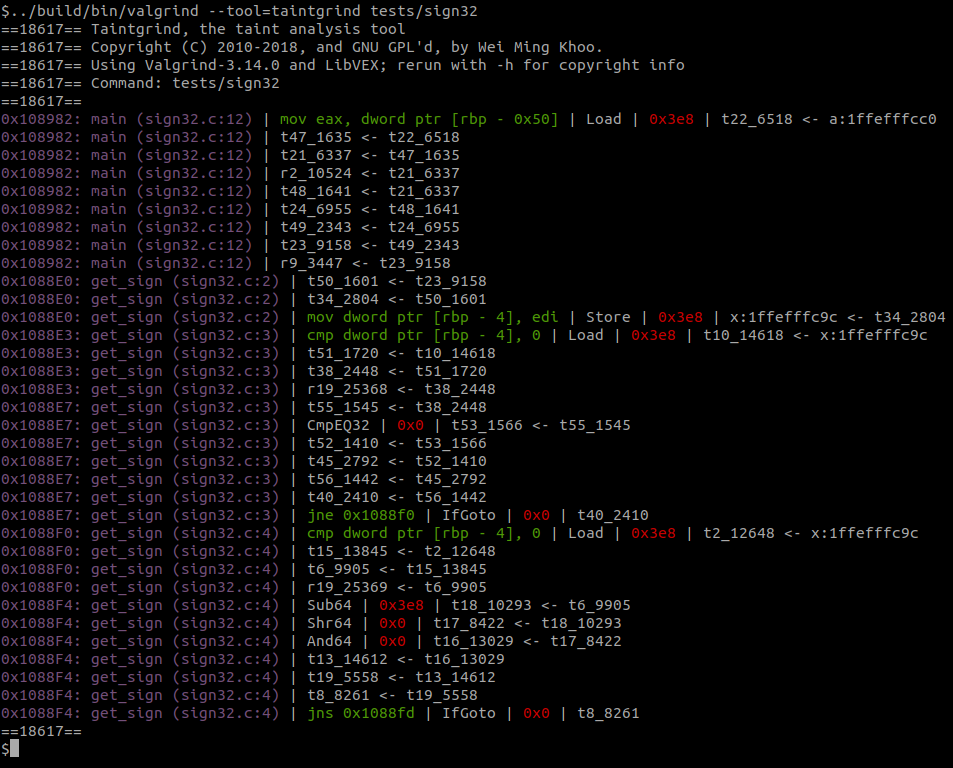
\includegraphics[scale=0.5]{img/taintgrind.png}
    }
    \caption{Пример работы Taintgrind}
    \label{fig:taintgrind}
\end{figure}

Также как и Triton, taintgrind отслеживает только сам факт помеченности данных, не различая источники, что делает его неприменимым для поставленной задачи.

\subsection{libdft}

Libdft -- инструмент для динамического анализа потока данных, представленный в \cite{libdft}. Оригинальная версия libdft поддерживает только x86 архитектуру. Однако в проекте Vuzzer \cite{vuzzer} используется модифицированная версия libdft64, поддерживающая x86\_64 Linux. Поскольку в данной работе исследуется анализ 64битных приложений интерес представляет именно 64битная версия.
Для инструментации libdft использует фреймворк Pin версии $3.7$\footnote{С 2019 года, ранее использовалась версия $2.14$}


% According to the paper[10] libdft provides file inputs as taint sources, but as we discovered libdft provides only syscall hooks. This tool provides to developer a classical taint engine. Libdtf uses byte-level tagging granularity. Taint tags are stored in flat bitmap. It requires only 384MB of contiguously memory to store all possible tags for 32bit Linux systems. For 64bit systems flat bitmaps is not reasonable, because it would require 32TB of memory to store taint tags. Libdft do not supports SSE and MMX instruction set.

libdft предоставляет API для установки обработчиков следующих событий
\begin{itemize}
    \item \texttt{syscall\_set\_pre} --- Установка обработчика перед системным вызовом;
    \item \texttt{syscall\_set\_post} --- Установка обработчика после системного вызова;
    \item \texttt{ins\_set\_pre} --- Установка обработчика перед выполнением инструкции;
    \item \texttt{ins\_set\_post} --- Установка обработчика после выполнения инструкции;
\end{itemize}
А также API для извлечения информации о пометках. Кроме того, есть возможность использовать возможности непосредственно Pin.

Оригинальный Libdft использует концепцию теневой памяти, для одного байта памяти инструментируемого приложения резервируется 1 байт в теневой памяти, позволяюший хранить информацию о 8 источниках пометок. Для снижения накладных расходов теневая память хранится постранично и её аллоциирование и удаление производится синхронно с памятью инструментируемого приложения.
В libdft64 для хранения информации о метках также используется библиотека сжатых битовых векторов EWAHBoolArray, что позволяет хранить более 8 пометок.

В оригинальном libdft отсутствует возможность помечать данные только из конкретного файла, есть только возможность указать что считать источником помеченных данных: файловую систему, стандартный ввод или сеть.
В libdft64 поддерживается только файловая система.

При распространении пометки учитывается семантика инструкции и тип её операнда, что способствует точности распространения пометок. Однако в libdft отсутствует поддержка регистра флагов\footnote{Разработчики сочли его ненужным, поскольку зависимости по управлению не учитываются}, а также SSE инструкций.

\subsection{Moflow gentrace}

Moflow -- это фреймворк для обнаружения поиска уязвимостей в исполняемых файлах, разработанный в Cisco Talos \cite{moflow}. Он использует BAP (Binary Analysis Platform) и Intel Pin для снятия трасс выполнения.
А также содержит утилиты:
\begin{itemize}
    \item \texttt{EGAS} --- инструмент автоматической генерации тестов, основанный на динамическом символьном выполнении. Аналог SAGE от Microsoft.
    \item \texttt{SLICER} --- Инструмент для прямого и обратного слайсинга по трассе
\end{itemize}

Для целей работы интерес представляет утилита \texttt{gentrace}, являющаяся также частью BAP. BAP написан на OCaml. Сам gentrace это основанный на Pin инструмент, написанный на С++, однако для своей работы он использует Ocaml библиотеки и protobuf, из-за подобной зависимости gentrace основывается на старой версии pin $2.14$.

\texttt{gentrace} не только позволяет сохранять трассы выполнения многопоточных программ, но также может снабдить их информацией о помеченных данных. Поддерживается возможность помечать аргументы командной строки, данные из конкретного файла, данные из стандартного потока ввода, а также данные из переменных окружения.
Кроме того присутствует поддержка всего набора инструкций X86\_64.

К недостаткам инструмента можно отнести то, что не смотря на побайтовую гранулярность меток, конкретной ячейки памяти может соответствовать только одна метка. Информация о пометках хранится в двух хэш таблицах. В первой из них ключами являются регистры, а во второй адреса из адресного пространства анализируемого процесса, ключами являются значения меток. 
Для хранение информации о метке используются беззнаковые 32битные числа, при этом
\begin{enumarate}
    \item $0$ Обозначает, что данные не помечены
    \item $2^{32} - 1$ обозначает, что данные помечены более чем одной меткой
    \item Другие числа обозначают непосредственно номер метки, соответствующий адресу или регистру.
\end{enumarate}

\subsection{Angr}

\texttt{Angr} -- это фреймворк для анализа исполняемых файлов, написанный на Python \cite{Angr}. Использует VEX в качестве языка для промежуточного представления, благодаря чему поддерживает все платформы, поддерживаемые Valgrind.
Angr реализует онлайн подход к динамическому символьному выполнению. Он также использует библиотеки \texttt{claripy} в качестве фронтенда к SMT-решателю и \texttt{cle} в качестве загрузчика.

API Angr построено на высокоуровневых абстракциях. Основными сущностями являются
\begin{itemize}
    \item \texttt{Project} ~--- класс инкапсулирующий в себе исследуемый исполняемый файл.
    \item \texttt{Block} ~--- класс представляющий базовый блок.
    \item \texttt{State} ~--- класс представляющий состояние исполняемого процесса.
    \item \texttt{Simulation Manager} ~--- класс, управляющий выполнением программы. В частности, предоставляет метод \texttt{step}, позволяющий пошагово производить вычисления.
\end{itemize}

Также Angr предоставляет набор так называемых Анализов, классов реализующих интерфейс \texttt{Analysis}. В частности, анализы позволяют построить граф потока управления (CFG) и граф зависимостей по данным (DDG), выполнить обратный слайсинг и найти адреса библиотечных функций.

Кроме того, Angr поддерживают такую абстракцию как ``Символьный файл'', вместо того, чтобы перехватывать системные вызовы и помечать прочитанные байты можно создать объект класса \texttt{SymbolicFile}. Его содержимому изначально соответствует массив из символьным битов, который и будет использоваться в случае чтения файла.

Кроме того присутствует возможность установить обработчики на различные внутренние события, такие как например чтение определенного адреса памяти или добавление новой формулы в предикат пути.

Несмотря на вышеперечисленные достоинства, Angr не лишен недостатков. С точки зрения данной работы, наиболее серьезным минусом является невозможность конкретного выполнения. Angr не выполняет процесс на реальном или виртуальном процессоре, а интерпретирует оттранслированный в VEX код, при этом адресное пространство процесса формируется при помощи cle, соответствующий оригинальный код не используется. Для всех неиницелизированных значений регистров и памяти Angr по умолчанию создает символьные переменные\footnote{Существует также опция, позволяющая считать их 0}. Для некоторых библиотечных функций их семантика эмулируется\footnote{Есть возможность отключить эту опцию, а также добавлять пользовательские функции для эмуляции}. Аналогичным образом происходит эмуляция системных вызовов.


Angr также предоставляет интерфейс \texttt{ExplorationTechique}, управляющий обходом графа и ряд его реализаций. Ниже перечислены некоторые из них

\begin{itemize}
    \item \texttt{DFS} ~--- Использует обход в глубину
    \item \texttt{Explorer} ~--- Техника, использующаяся по умолчанию. Позволяет указать адреса, которые следует найти, а также адреса которых следует избегать (если такой адрес встретился, то соответствующая ветка дальше в глубину не исследуется). Вместо адреса также можно задать предикат, который будет вычисляться на каждом адресе.
    \item \texttt{Tracer} ~--- Следует трассе, снятой при помощи QEMU.
    \item \texttt{Symbion} ~--- Использует конкретное выполнение в отдельном процессе (под GDB) синхронизируя значения в обе стороны.
\end{itemize}

К сожалению, две последние техники работают нестабильно, попытки использовать их как есть не увенчались успехом, так в случае \texttt{Tracer} адреса базовых блоков полученных из qemu не соответствуют адресам. Техника \texttt{Explorer} успешно отработала на нормальных примерах, но не смогла достигнуть заданных адресов на реальном приложении (в частности \texttt{cmark}).


\subsection{Manticore}

\texttt{Manticore} \cite{trailofbits-manticore}~-‑- Это библиотека для динамического символьного выполнения для анализа исполняемых ELF файлов для ARM, x86 и x86-64 Архитектур. Он также поддерживает смарт контракты для \texttt{Etherium} (EVM байткод).

Авторы позиционируют Manticore как простой аналог Angr c меньшей кривой обучения. C точки зрения задачи, рещаемой в данной работе основным преимуществом является возможность конкретного выполнения.

При этом инструмент имеет следующие недостатки:

\begin{itemize}
    \item Нет возможности устанавливать обработчики на системные вызовы.
    \item Некоторые системные вызовы не поддерживаются
    \item SSE инструкции не поддерживаются
    \item Медленная скорость эмуляции (50 секунд на код до main в приложении использующем glibc)
\end{itemize}



% \section{Динамическое символьное выполнение}


% \subsection{Triton}

% \subsection{angr}

% \subsection{manticore}



% \chapter{Сравнение инструментов для динамического анализа}

% \section{Библиотека для снятия и анализа трас}

% \section{Результаты сравнение}

% \section{Выводы}






% \chapter{Выбор технологии для реализации}

% \section{Библиотека для снятия и анализа трас}

% \section{Результаты сравнение}


% \chapter{Реализация}


% \section{Решение на основе Moflow}

% \chapter{Заключение}
% \subsection 




 % Для решения этой проблемы может использоваться динамическое символьное выполнение, например Driller для фаззера afl \cite{DRILLER}. Для улучшения работы фаззера